\section{METHODOLOGY}
% \subsection{Project Timeline}
% Timeline for our project is as shown in Figure \ref{fig:ganntt}.
% \begin{figure}[h!]\centering
%   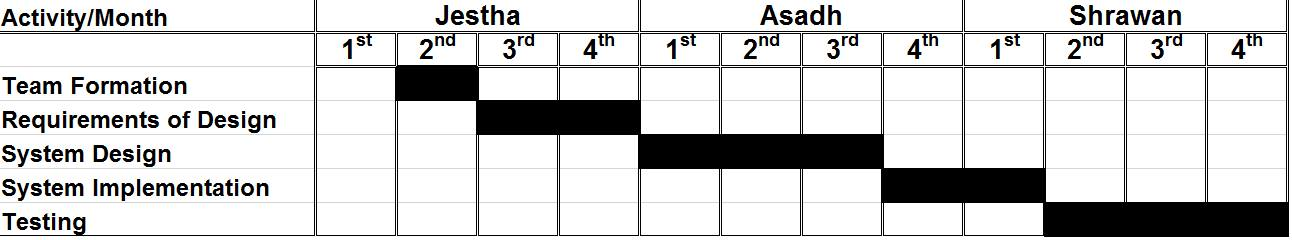
\includegraphics[width=6in]{fig/ganntt}
%   \caption{Gantt chart of project development }\label{fig:ganntt}
% \end{figure}
\subsection{Data Collection}
Both analysis and prediction of stock market needed an extensive amount of data for better visualization and training. News data regarding stock market were required for news analysis, which were collected from sharesansar website via web crawling. Trading data of listed companies, for technical analysis were collected from merolagani website. Similarly, Sector wise data required for Nepal Stock Exchange Ltd.(NEPSE)  index prediction were collected from sharesansar. Unfortunately, the data required for Fundamental Analysis were not available for crawling. As a result, required data were extracted manually from the web.\\

Aside from the static past data, a mechanism to update the recent changes was also required to update the database constantly. For this, a manual update module was built, which at the end of the day, updates the changes made throughout the day in the database

\subsection{Data Preprocessing}
The trading data crawled from Merolagani and Sharesansar had numerous missing fields, which were  filled up using interpolation technique to cover up the possible setbacks. Once the data is cleaned, it is stored in the database for future retrievals.\\

The training data on analysis showed high fluctuation, which needed some smoothing technique in order to feed it into our model for better results. Thus, Exponential Moving Average was used to reduce the data into suitable form.\\

For the news analysis, the news so collected are to be divided into feature set and label. The feature set were extracted using 'Bag of words representation'. The label were given to each vector as positive or negative based on whether the corresponding price increased or decreased .All the news were labeled accordingly to get a complete training data set.

\subsection{Data analysis and visualization}
Data Analysis in financial market involves two basic approaches and they are: Technicalanalysis and Fundamental analysis. Technical analysis, which involves detecting patterns in security prices, goes on the assumption that the price of a stock - like the price of everything
else - is a matter of supply and demand. Technical analysis generates and interprets charts of the price and volume histories of stocks to predict movement in stock prices according to perceived trends. Fundamental analysis, which examines the earning potential of the company issuing a stock, goes on the assumption that a share of ownership of a company has anintrinsic value that is a function of the underlying value of the company as a whole. Fundamental analysis reports which shares are undervalued by the investor community and which are overvalued then trust the market to make corrections.\\

Data visualization is a general term that describes any effort to help people understand the significance of data by placing it in a visual context. Data visualization was done with the help of charting library called AmCharts. Company wise data were shown in charts and features like comparison of stock data were also integrated.

\subsection{Feature Selection}
The data features that are used to train  machine learning models have a huge influence on the performance that can be achieved. Irrelevant or less relevant selection of data features result in low performance during prediction. So, it is necessary to select the best possible features that best influence the result.\\

Benefits of performing feature selection before modeling the data are:
\begin{itemize}
	\item Reduces Over-fitting: Less redundant data means less opportunity to make decisions based on noise. 
	\item Improves Accuracy: Less misleading data means modeling accuracy improves. 
	\item Reduces Training Time: Less data means that algorithms train faster. 
\end{itemize}

Statistical tests can be used to select those features that have the strongest relationship with the output variable. The scikit-learn library provides the SelectKBest class that we used with a suite of different statistical tests to select a specific number of features.

\subsection{Prediction}
The system intends to predict the stock market using the available historical data. The prediction model is generated by manipulating the historical data by casting them through various artificial intelligence techniques. In general, stock market prediction can be done by analyzing the past stock trends with respect to fundamental, technical and news-sentiment analysis. 
\subsubsection{Prediction using Technical Analysis }
[1]The field of technical analysis is based on three assumptions:\\
	a. The market discounts everything\\
	b. Price moves in trends\\
	c. History tends to repeat itself\\
Technical analysis studies the trend of supply and demand within the market to determine what direction or trend will continue in the future. In other words, it attempts to understand the emotions in the market by studying the market itself, as opposed to its components. Various technical indicators, such as Relative Strength Index (RSI) and Moving Average Convergence Divergence (MACD), are used to ease the process of technical analysis. 

\chapter{\textbf{1. Technical analysis using Artificial Neural Network  }}\\
Artificial Neural Networks (ANNs) are simply inspired from biological neural networks that make up the networks of living neuron cells in animals. Computer systems excel the human brain in performing complex mathematical operations by thousands of times but, lack the human ability of logical reasoning and pattern recognition. The use of ANN allows computers to process data the same way the human brain processes a stimulus, providing them the ability to recognize patterns even in non-linear data such as that of stock market. For this process, the ANN is trained with historical data using supervised learning method. Once the training is completed, we move on to the testing phase, where the reliability, accuracy and efficiency of the training algorithm is tested. Once the ANN has passed the test, it can then be used for prediction. 

%The artificial neural network model is shown in Figure \ref{fig:NN}
\begin{figure}[h!]\centering
	%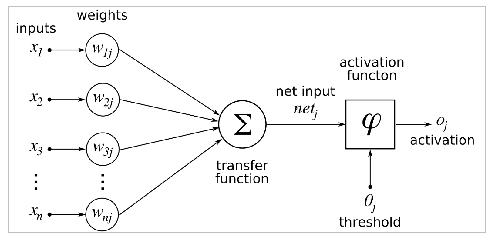
\includegraphics{fig/NN.png}\\[0.2cm]
	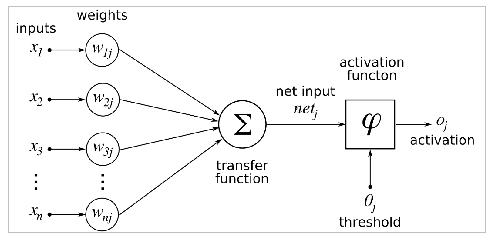
\includegraphics[width=5in]{fig/NN}
  
	\caption{ANN model }\label{fig:NN}

   %\caption{Gantt chart of project development }\label{fig:ganntt}
 \end{figure}

ANN is considered one of the most effective methods in predicting the stock market. Even within ANN, the Multi-Layer Perceptron (MLP) model is widely accepted for effective pattern recognition. [2] An MLP model is a class of feed-forward Artificial Neural Network that consists of at least three layers of nodes namely: Input layer, Hidden layer(s) and Output layer. MLP utilizes supervised learning technique and Backpropagation algorithm for training.

The artificial neurons shown in \ref{fig:NN} have n number of inputs: \[x_1, x_2,...,x_n\] each of which is associated with a weight onto the connection line, denoted as \[w_1_j, w_2_j,...,w_n_j\] respectively. The weights can be referred as synaptic weights as in a biological neural network. "\theta  \]"  represents the threshold and "\alpha  \]" represents the activation function given by:

\alpha = \sum_{k = 1}^{n} [ w_k_j * x_k + \theta]

The output of the neuron, Oj, is a function of its activation given by:
O_j = f(\alpha)

Several types of activation functions can be used, which are summarized in Figure \ref{fig:NNtable}:
\begin{figure}[h!]\centering
	
	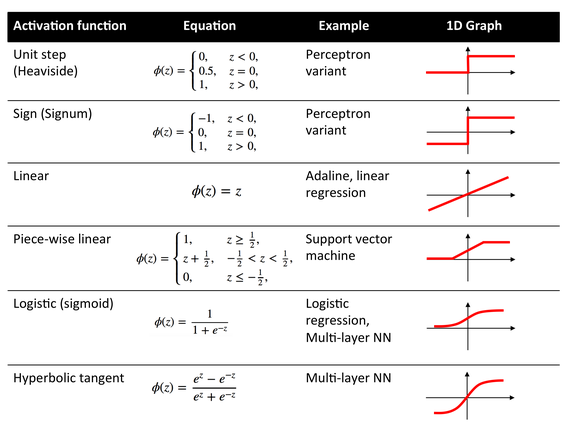
\includegraphics[width=4in]{fig/NNtable}
  \caption{Table showing activation function}\label{fig:NNtable}

    \end{figure}

\chapter{\textbf{2. Backpropagation Algorithm }}\\
The chief objective of the Backpropagation Algorithm is to reduce the error function. [3] This algorithm falls into the general category of gradient descent algorithms, which intend to find the minima/maxima of a function by iteratively moving in the direction of the negative of the slope of the function to be minimized/maximized. This algorithm proceeds across the network, providing activation to each node until the output node is reached. Then, the weights are updated backwards, from the output layer towards the input layer until one epoch has been completed. The weights are updated according to the respective errors computed for each layer. 

\begin{figure}[h!]\centering
	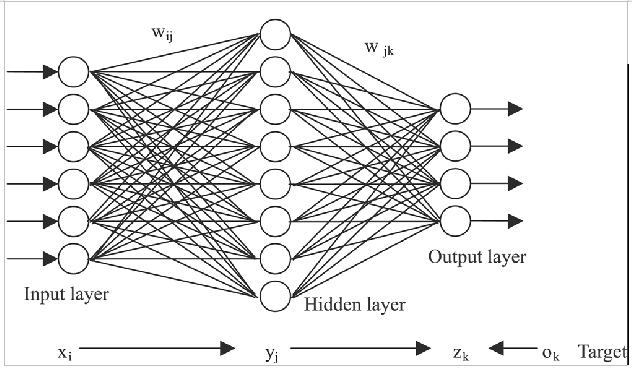
\includegraphics[width=4in]{fig/back}
	\caption{Backpropagation Algorithm}\label{fig:back}
\end{figure}

In the figure \label{fig:back}, For k output units, if t_{k} \]  signifies the target value, o_{k} \] signifies the actual output, \alpha \] signifies the learning rate and z_{ink} \] signifies the activation function for the k^{th} \] output node, error (\delta \]) is given by:
\delta_k = (t_k - o_k) * f\'(z_{ink}) 

Now, the weight correction for each output unit is given by:
${\Delta}$ w_{jk} = \alpha * \delta_{k} * z_{j} \]

Similarly, by propagating the delta term further back in the network, the input error in the hidden network is calculated
	\delta_{inj} = \sum_{k =1}^{m}  \delta_k * w_{jk} \]
Where, m = number of neurons in the hidden layer

Now, error in the jth hidden unit is calculated by:
	\delta_j = \delta_{inj} * f\'(x_{inj} \])
Where x_{inj} \] signifies the activation function for the j^{th} \] hidden layer node.

Now, the weight correction is given by:

${\Delta}$ w_{ij} = \alpha * \delta_j * X_i \] 	, for hidden layer nodes\\
${\Delta}$ w_{jk} = \alpha * \delta_k * Y_j \]	, for output layer nodes

Then, the weights for each neuron is updated with the new ones. Once an epoch has been completed, the average error for each training data is calculated. Usually the RMS error between the target value and actual outputs is computed for convergence. If the RMS error falls within the acceptable range, the training is completed, else, the whole process is repeated.

Hence, the above algorithm can be used to train an Artificial Neural Network. The network, in general, can have an arbitrary number of hidden layers and an arbitrary number of hidden neurons in each layer. For practical reasons, ANNs implementing the backpropagation algorithm do not have too many layers, since the time for training the networks grows exponentially. The number of input layer neurons is decided by the number of input features in each pattern, and the number of output layer neurons is decided by the number of output features in the target values.  

There are a few disadvantages associated with backpropagation learning as well: 
\begin{itemize}
 \item The convergence obtained from backpropagation learning is very slow. 
\item The convergence in backpropagation learning is not guaranteed. 
\item The result may generally converge to any local minimum on the error surface, since stochastic gradient descent exists on a surface which is not flat. 
\item Backpropagation learning requires input scaling or normalization. 
\item Backpropagation requires the activation function used by the neurons to be differentiable.
\end{itemize}

\subsubsection{K- nearest neighbor}
The k-nearest neighbors algorithm is a non-parametric method used for classification and regression. We are using k-NN for classification of news in news  analysis in our project. The input consists of the k closest training examples in the feature space. The output in k-NN classification is a class membership. An object is classified by a majority vote of its neighbors, with the object being assigned to the class most common among its k nearest neighbors. The K-Nearest Neighbor  is a simple lazy learner algorithm that stores all available data points  and classifies new instances based on a similarity measure.

\begin{figure}[h!]\centering
	
	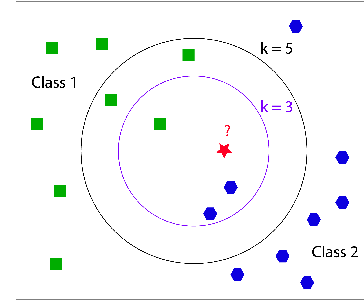
\includegraphics[width=4in]{fig/KNN}
  \caption{KNN model}\label{fig:KNN}

    \end{figure}
    
During the training phase the algorithm simply stores the data points including their class labels and all computation is deferred until the classification process. It is based on a principle that instances that are in close proximity to another have similar properties. Thus, to classify new unclassified instances, one simply has to look at their k-nearest neighbors, to figure out  the classification label. The class membership can be defined by a majority vote of the k closest neighbors or the neighbors can be ranked and weighted according to their distance to the new instance.

\subsection{Tools and Technique}
The various tools and techniques used in this project are described below: \\
%\subsubsection{Tools}
\chapter{\textbf{1.Python }}\\
The whole project is written in Python Programming Language. Various libraries of python are used in the project. Python is a general-purpose interpreted, interactive, object-oriented, and high-level programming language. It was created by Guido van Rossum during 1985- 1990. Like Perl, Python source code is also available under the GNU General Public License (GPL). \\

Python is designed to be highly readable. It uses English keywords frequently where as other languages use punctuation, and it has fewer syntactical constructions than other languages. Python is processed at runtime by the interpreter. Python is Interactive. Users can actually sit at a Python prompt and interact with the interpreter directly to write programs. Python is Object-Oriented: Python supports Object-Oriented style or technique of programming that encapsulates code within objects. Python is a Beginner's Language: Python is a great language for the beginner-level programmers and supports the development of a wide range of applications from simple text processing to WWW browsers to games. It supports functional and structured programming methods as well as OOP. It can be used as a scripting language or can be compiled to byte-code for building large applications. It provides very high-level dynamic data types and supports dynamic type checking. It supports automatic garbage collection. It can be easily integrated with C, C++, COM, ActiveX, CORBA, and Java. 

\chapter{\textbf{2. Pandas }}\\
Pandas is a software library written for the Python programming language for data manipulation and analysis. In particular, it offers data structures and operations for manipulating numerical tables and time series. Pandas is free software released under the three-clause BSD license. The name is derived from the term "panel data", an econometrics term for multidimensional structured data sets. Python has long been great for data munging and preparation, but less so for data analysis and modeling. Pandas helps fill this gap, enabling users to carry out the entire data analysis workflow in Python without having to switch to a more domain specific language like R. Pandas modules uses objects to allow for data analysis at a fairly high performance rate in 
comparison to typical Python procedures. With it, users can easily read and write from and to CSV files, or even databases. From there, users can manipulate the data by columns, create new columns, and even base the new columns on other column data.

\chapter{\textbf{3. Scikit learn }}\\
Scikit-learn (formerly scikits.learn) is a free software machine learning library for the Python programming language. It features various classification, regression and clustering algorithms including support vector machines, random forests, naive bayes, gradient boosting, k-means and DBSCAN, and is designed to inter operate with the Python numerical and scientific libraries NumPy and SciPy. Scikit-learn was initially developed by David Cournapeau as a Google summer of code project in 2007. Later Matthieu Brucher joined the project and started to use it as apart of his thesis work. In 2010 INRIA got involved and the first public release (v0.1 beta) was published in late January 2010. Scikit-learn provides a range of supervised and unsupervised learning algorithms via a consistent interface in Python. It is licensed under a permissive simplified BSD license and is distributed under many Linux distributions, encouraging academic and commercial use. 
Some popular groups of models provided by scikit-learn include: 
\begin{itemize}
	\item Clustering: for grouping unlabeled data such as KMeans.
	\item Cross Validation: for estimating the performance of supervised 	models on unseen data.
	\item Dimensionality Reduction: for reducing the number of attributes in data for summarization, visualization and feature selection such as Principal component analysis. 
	\item Feature extraction: for defining attributes in image and text data. 
	\item Parameter Tuning: for getting the most out of supervised models. 
	\item Supervised Models: a vast array not limited to generalized linear models, discriminate analysis, naive bayes, lazy methods, neural networks, support vector machines and decision trees. 
\end{itemize}

\chapter{\textbf{4.Numpy }}\\
Numpy is  the core library for scientific computing in Python.NumPy is a Python package. It stands for 'Numerical Python'. It is a library consisting of multidimensional array objects and a collection of routines for processing of array.\\

Using NumPy, a developer can perform the operations like Mathematical and logical operations on arrays, Fourier transforms and routines for shape manipulation, Operations related to linear algebra, NumPy has in-built functions for linear algebra and random number generation.\\

\chapter{\textbf{5.NLTK }}\\
NLTK is a leading platform for building Python programs to work with human language data. It provides easy-to-use interfaces to over 50 corpora and lexical resources such as WordNet, along with a suite of text processing libraries for classification, tokenization, stemming, tagging, parsing, and semantic reasoning. Tokenizers is used to divide strings into lists of substrings. For example, Sentence tokenizer can be used to find the list of sentences and Word tokenizer can be used to find the list of words in strings.NLTK is one of the natural language processing tool that was used in the project.\\

\chapter{\textbf{6. Django}}\\
Django was used in the project to design the web interface. Django is a free and open-source web framework, written in Python, which follows the modelcontroller (MVC) architectural pattern. It is maintained by the Django Software Foundation (DSF), an independent organization established as a 501(c)(3) non-profit. Django's primary goal is to ease the creation of complex, database-driven websites. Django emphasizes reusability and "pluggability" of components, rapid development, and the principle of don't repeat yourself.\\
 
Python is used throughout, even for settings files and data models. Django also provides an optional administrative create, read, update and delete interface that is generated dynamically through introspection and configured via admin models. 

\chapter{\textbf{7.Git}}\\
Git was used as a version control system to collaborate among the team members. Git is a version control system that is used for software development and other version control tasks. As a distributed revision control system it is aimed at speed, data integrity, and support for  distributed, non-linear workflows. Git was created by Linus Torvalds in 2005 for development of the Linux kernel, with other kernel developers contributing to its initial development. The Git feature that really makes it stand apart from nearly every other SCM out there is its branching model. \\

Git allows and encourages you to have multiple local branches that can be entirely independent of each other. The creation, merging, and deletion of those lines of development takes seconds.\\

\chapter{\textbf{8.Postgresql}}\\
PostgreSQL is a powerful, open source object-relational database system. It has more than 15 years of active development and a proven architecture that has earned it a strong reputation for reliability, data integrity, and correctness. PostgreSQL runs on all major operating systems, including Linux, UNIX (AIX, BSD, HP-UX, SGI IRIX, Mac OS X, Solaris, Tru64), and Windows. PostgreSQL (pronounced as post-gress-Q-L) is an open source relational database management system (RDBMS) developed by a worldwide team of volunteers. PostgreSQL is not controlled by any corporation or other private entity and the source code is available free of charge. It supports text, images, sounds, and video, and includes programming interfaces for C / C++, Java, Perl, Python, Ruby, Tcl and Open Database Connectivity (ODBC). PostgreSQL supports a large part of the SQL standard and offers many modern features like Complex SQL queries, SQL Sub-selects, Foreign keys, Trigger, Views, Transactions, Multiversion concurrency control (MVCC), Streaming Replication (as of 9.0), Hot Standby (as of 9.0).

\chapter{\textbf{9.AM Charts (JavaScript Charts)}}\\
AM Charts made it easy to display complex data visualizations. Combine various graph types on a single chart. Create clusters, or stacks, or clusters of stacks. Control the widths,open and close values, apply coloring based on value thresholds or changes, recalculate the values automatically. Use various value scales, including date and time. Those are just a few examples of what we can do.

\subsection*{Features of AM Charts}
\begin{itemize}
	\item \textbf{Interactive}\\
Zoom or pan serial charts, drill-down to other data levels, select slices, toggle graphs using legend, display HTML-rich contextual info, or draw trend lines directly on chart.
	\item \textbf{Export options}\\
Annotate and export charts dynamically to various formats including static images, SVG, PDF, Excel, and CSV.
	\item \textbf{Load external data}\\
Easily setup and load external data sources in JSON or CSV formats. Enable reloads. Add custom pre-processing functions.
	\item \textbf{Extendable}\\
Enhance charting capabilities with a range of plugins built by amCharts team.
	\item \textbf{Responsive}
Resize your browser window, rotate the phone, watch the chart not just take the new shape, but adapt its contents and controls accommodate available space. Use full-fledged responsive features transparently, or write your own responsive rules.
	\item \textbf{Mobile-friendly}\\
We made it extremely easily control the charts using touch gestures. Zoom, pan, click the charts, without sacrificing the general responsiveness of the web page.
	\item \textbf{Accessible}\\
As of version 3.20 JavaScript Charts features extensive accessibility functionality right out-of-the-box. The product is fully compatible with standard-based screen readers as well as W3C-approved properties for easy navigation between map elements for people with impaired vision or with mobility restrictions. The screen reader content is even customizable per your requirements. Visit our Accessibility center for more information.
	\item \textbf{Dynamic}\\
Update data, size or just about any other configuration variable dynamically, without reloading the page. Add graphs, legends, titles, guides, bullets, or change colors, switch between 3D settings on the fly via well-documented API. Tap into chart\'s various events using custom handler functions.
	\item \textbf{Live-updated charts}\\
Update data every second to create `live' charts. Simulate just about any interaction using API function calls.
\end{itemize}

